\newpage
\chapter{DISEÑO DEL SISTEMA DE INFORMACIÓN}
	\vspace{2cm}	
	\begin{center}
	{\Large \textbf{FASE DE DESARROLLO} \par}
	\end{center}
	\vspace{5cm}
	
	\begin{center}
	\Huge \textbf{DSI}\par
	\end{center}

\newpage


\section{DSI 3: DISEÑO DE CASOS DE USO REALES}

\subsection{Caso de Uso 1.1} 

\subsubsection{Diagramas de Interacción (Comunicación y Secuencia)} 

\subsubsection{Diagramas de Estados de las Clases} 
 
\subsubsection{Diagramas de Actividades} 


\subsection{Caso de Uso 1.2}


\newpage
\section{DSI 4: DISEÑO DE CLASES}

\subsection{Diagrama de Clases}


\newpage
\section{DSI 5: DISEÑO DE LA ARQUITECTURA DE MÓDULOS DEL SISTEMA}

\subsection{DSI 5.1 Diseño de Módulos del Sistema}

\subsection{DSI 5.2 Diseño de Comunicaciones entre Módulos}

\subsection{DSI 5.3 Revisión de la Interfaz de Usuario}


\newpage
\section{DSI 6: DISEÑO FÍSICO DE DATOS}

\subsection{Descripción del SGBD Usado} 
Se ha creado una base de datos relacional, utilizando MySQL 8 como sistema gestor de bases de datos, debido a su gran popularidad en todo el mundo y, más concretamente, en entornos de desarrollo web.\\
\par {\color{red}explicar algo más}

\subsection{Integración del SGBD en Nuestro Sistema} 

\subsection{Diagrama E--R} 
\begin{figure}[H]
\centering
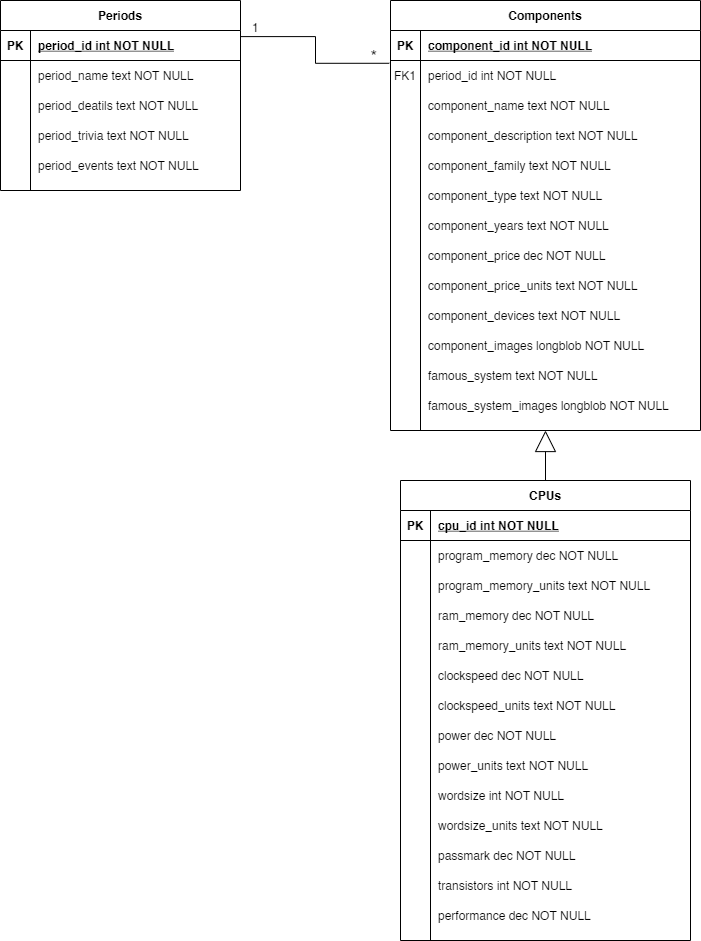
\includegraphics[scale=0.6]{diagrama_e-r}
\caption{Diagrama Entidad-Relación de la base de datos creada}
\end{figure}

\newpage
\section{DSI 9: DISEÑO DE LA MIGRACIÓN Y CARGA INICIAL DE DATOS}


\newpage
\section{DSI 10: ESPECIFICACIÓN TÉCNICA DEL PLAN DE PRUEBAS}

\subsection{Pruebas Unitarias} 

\subsection{Pruebas de Integración y del Sistema} 

\subsection{Pruebas de Usabilidad y Accesibilidad} 

\subsubsection{Diseño de Cuestionarios} 

\subsubsection{Actividades de las Pruebas de Usabilidad} 


\subsection{Pruebas de Accesibilidad} 

\subsection{Pruebas de Rendimiento} 
